%#BIBTEX pbibtex paper
%\documentclass[preprint]{ptephy_v1}
\documentclass{ptephy_v1}
%%%%%%%%%%%%%%%%%%%%%%
\usepackage{latexsym,graphicx,amssymb,amsmath,mathrsfs}
\usepackage{epstopdf}
\usepackage{url}
\graphicspath{{./Figs/}}
\newcommand{\LL}{\Lambda\Lambda}
\newcommand{\nuc}[2]{{}^{#1}\mathrm{#2}}
\newcommand{\nucL}[2]{{}^{#1}_\Lambda\mathrm{#2}}
\newcommand{\nucLL}[2]{{}^{#1}_{\LL}\mathrm{#2}}
%%%%%%%%%%%%%%%%%%%%%%

\newcommand\APF{\langle{e^{i\theta}}\rangle_\mathrm{pq}}
\newcommand\vev[1]{\langle #1 \rangle}
\newcommand\Pbar{\overline{P}}
\newcommand{\QCDone}{0+1D QCD}
%\newcommand{\QCDone}{$\mathrm{QCD}_{0+1}$}
%
%\usepackage[usenames]{color}
\usepackage[normalem]{ulem}  % \sout{old text} for strikeout
\newcommand{\com}[1]{{\color[rgb]{0,0,1}{#1}}}
\newcommand{\comm}[1]{{\color[rgb]{1,0,1}{#1}}}
\newcommand{\AO}[1]{{\color[rgb]{0,0.3,0}{#1}}}
\renewcommand\sout{\bgroup \color{red} \ULdepth=-.5ex \ULset}


\begin{document}

\preprintnumber{YITP-19-??}

\title{
Statistical decay of double $\Lambda$ compound nuclei
and hyperfragment fomation
from $\Xi^-$ absorption at rest on nuclei
}

\author[1]{Akira Ohnishi}
\affil{Yukawa Institute for Theoretical Physics, Kyoto University,
Kyoto 606-8502, Japan
\email{ohnishi@yukawa.kyoto-u.ac.jp}}

\author[2]{Chikako Ishizuka}
\affil{TITech}

\author[2]{Kohsuke Tsubakihara}

\author[3]{Yuichi Hirata}
\affil{Hokkaido University}

\begin{abstract}
To be written
\end{abstract}

\maketitle

\section{Introduction}
{\em General introduction:}
Double $\Lambda$ hypernuclei provide us with precious information 
on $\Lambda\Lambda$ interaction. ... (AO)
({\em Relevance to neutron star physics})
The $\LL$ interaction is also important in neutron stars.
Since most of the known $\Lambda N$ two-body interaction
leads to hyperon mixing in neutron star matter at $(2-4)\rho_0$
and also to softening of the equation of state (EOS),
it is not possible to support massive neutron stars with masses
around $2 M_\odot$ with $M_\odot$ being the solar mass.
Then it is necessary to find the mechanism to support massive neutron stars.
If the $\LL$ interaction is repulsive enough,
the softening of EOS does not proceed, and the EOS may be kept to be 
stiff enough. ... (Tsubakihara)


{\em Review of previous double hypernuclear formation (Exp. and Theor.):}
(Hirata)

{\em Recent double hypernuclear formation:}
(Ishizuka)

In this article, we discuss the formation of double $\Lambda$ hypernuclei
from the statistical decay of double $\Lambda$ compound nuclei
formed via the $\Xi^-$ absorption at rest on nuclei.
Specifically, we concentrate on the taret nuclei,
$\nuc{12}{C}$, $\nuc{14}{N}$ and $\nuc{16}{O}$.
These are the main light component of emulsion,
and some double $\Lambda$ hypernuclei have been reported to be formed.
We discuss the formation probabilities 
$\nucLL{6}{He}$ from $\Xi^-$ abosrption at rest on $\nuc{12}{C}$,
$\nucLL{13}{B}$ on $\nuc{14}{N}$ target,
and 
$\nucLL{11}{Be}$ on $\nuc{16}{O}$.
... (AO)

This paper is organized as follows.
...

\section{Statistical decay of double $\Lambda$ compound hypernuclei}
\label{Sec:theory}

Hirata-san, please.

%%%%%%%%%%%%%%%%%%%%
\begin{figure}[bthp]
\begin{center}
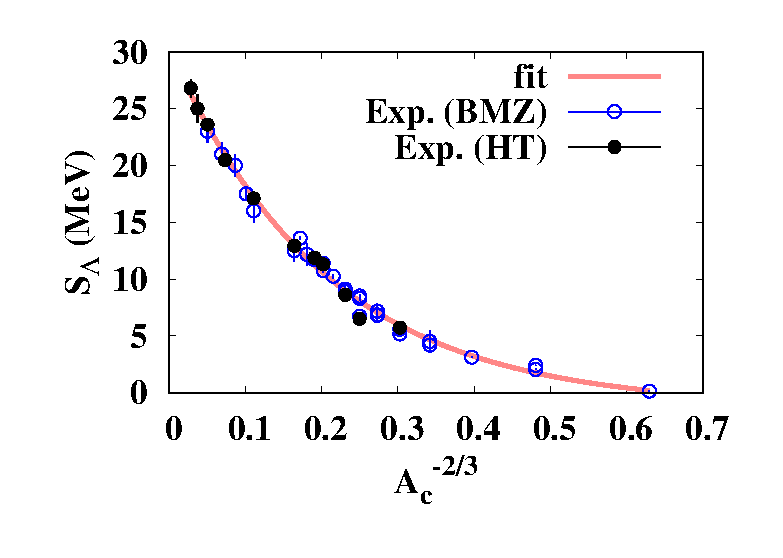
\includegraphics[width=0.5\textwidth]{SL.eps}%
\end{center}
\caption{
Separation energy of single hypernuclei.
Data summirized in \cite{BMZ} (blue open circles) and \cite{HT} (black filled circles)
are shown by symbols.
}
\label{Fig:SL}
\end{figure}
%%%%%%%%%%%%%%%%%%%%

\section{Double $\Lambda$ hypernuclear formation probabilities}
\label{Sec:results}

AO will do.

%%%%%%%%%%%%%%%%%%%%
\begin{figure}[htbp]
\begin{center}
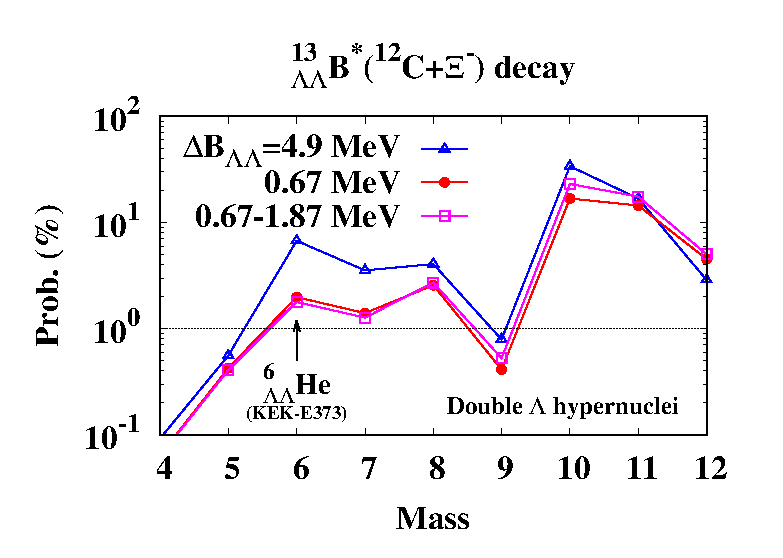
\includegraphics[width=0.5\textwidth]{C12Xi-cas.eps}%
\end{center}
\caption{
$^{12}\mathrm{C}+\Xi^-$
}
\label{Fig:C12Xi}
\end{figure}
%%%%%%%%%%%%%%%%%%%%

%%%%%%%%%%%%%%%%%%%%
\begin{figure}[htbp]
\begin{center}
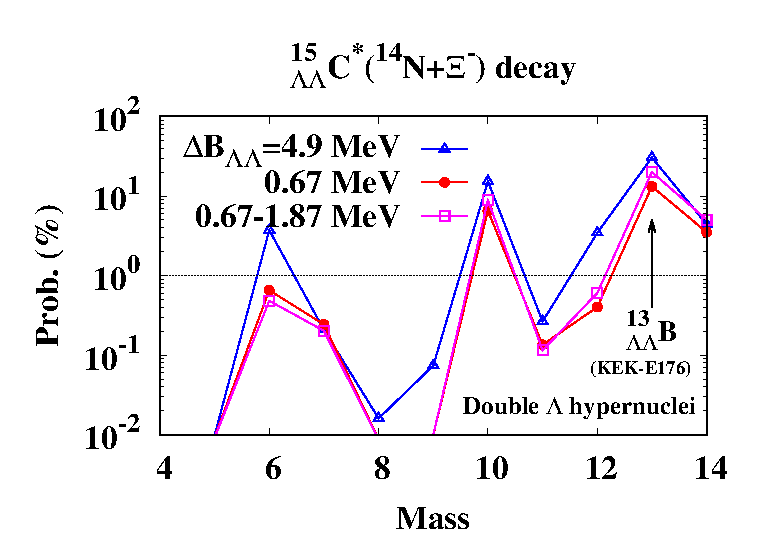
\includegraphics[width=0.5\textwidth]{N14Xi-cas.eps}%
\end{center}
\caption{
$^{14}\mathrm{N}+\Xi^-$
}
\label{Fig:N14Xi}
\end{figure}
%%%%%%%%%%%%%%%%%%%%

%%%%%%%%%%%%%%%%%%%%
\begin{figure}[htbp]
\begin{center}
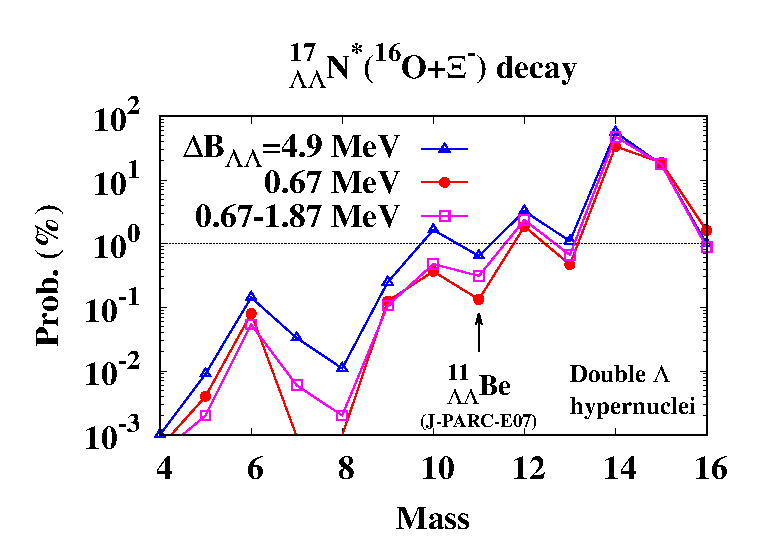
\includegraphics[width=0.5\textwidth]{O16Xi-cas.eps}%
\end{center}
\caption{
$^{16}\mathrm{O}+\Xi^-$
}
\label{Fig:O16Xi}
\end{figure}
%%%%%%%%%%%%%%%%%%%%


\section{Summary}
\label{Sec:Summary}

To be written.

\section*{Acknowledgments}
This work is supported in part by the Grants-in-Aid for Scientific Research
 from JSPS (Nos. 
%15H03663, % PI:Nakamura, with AO
%16K05350, % PI:Kunihiro, with AO
%18J21251, % Mori (JSPS)
%18K03618, % PI:Kashiwa
19H05151 %, % (Cluster) AO
and
19H01898), % Kiban B(Ohnishi, Kashiwa)
%
and by the Yukawa International Program for Quark-hadron Sciences (YIPQS).


\bibliographystyle{ptephy}
%\bibliography{ref}
\begin{thebibliography}{99}
\bibitem{BMZ}
%# BMZ: 
H. Bando, T. Motoba, J. Zofka, Int. J. Mod. Phys. 21 (1990), 4021-4198.

\bibitem{HT}
%# HT: 
O. Hashimoto, H. Tamura, Prog. Part. Nucl. Phys. 57 (2006), 564-653.
\end{thebibliography}

\end{document}
